\documentclass[11pt,letterpaper]{article}
\usepackage[utf8]{inputenc}

%----- Configuración del estilo del documento------%
\usepackage{epsfig,graphicx}
\usepackage[left=2cm,right=2cm,top=1.8cm,bottom=2.3cm]{geometry}
\usepackage{fancyhdr}
\usepackage{lastpage}
\usepackage{url}
\pagestyle{fancy}
\fancyhf{}
\rfoot{\textit{Página \thepage \hspace{1pt} de \pageref{LastPage}}}


%------ Paquetes matemáticos básicos --------%
\usepackage{amsmath}
\usepackage{amssymb}
\usepackage{amsthm}

\usepackage[spanish]{babel}
\usepackage{graphicx}
\usepackage{hyperref}

\usepackage{tabularx}
\usepackage{xcolor}
\usepackage[table]{xcolor}
\usepackage{colortbl}
\usepackage{array, multirow, multicol, tabularx}
\usepackage{tcolorbox}
\newtheorem{theorem}{Theorem}[section]
\newtheorem{corollary}{Corollary}[theorem]
\newtheorem{lemma}[theorem]{Lemma}

%------si-------%
\definecolor{B}{HTML}{FFFFFF}
\definecolor{G}{HTML}{5e5e5e}
\definecolor{R2}{HTML}{d53d40}
\definecolor{A2}{HTML}{034190}
\definecolor{V2}{HTML}{7faa50}
\newcommand{\R}{\mathbb{R}}
\newcommand{\C}{\mathcal{C}}
\newcommand{\Z}{\mathbb{Z}}
\newcommand{\Q}{\mathbb{Q}}
\newcommand{\N}{\mathbb{N}}
\renewcommand{\theenumi}{\Roman{enumi}}
\renewcommand{\labelenumi}{{\theenumi}.}

\begin{document}

%------ Encabezado -------- %

\begin{center}
    \begin{minipage}{3cm}
    	\begin{center}
    		\includegraphics[height=3.4cm]{esfm 1.png}
    	\end{center}
    \end{minipage}\hfill
    \begin{minipage}{10cm}
    	\begin{center}
    	
        \textbf{Concurso Pierre Fermat 2024}\\[0.1cm]
      El\'ias L\'opez Rivera  $^{1}$ \\[0.1cm]
       Jonathan Sayid Mercado Mart\'inez   $^{2}$\\[0.1cm] 
        \textbf{$^{1}$Facultad de Ciencias\,(UNAM)}\\[0.1cm]
        \textbf{$^{2}$ Escuela superior de F\'isica y Matem\'aticas\,(IPN)}\\[0.1cm]
        $^{1}$elias.lopezr@ciencias.unam.mx\\[0.1cm]
        $^{2}$jmercadom2000@alumno.ipn.mx \\[0.1cm]
        Fecha:\,\,19/05/2025
    	\end{center}
    \end{minipage}\hfill
    \begin{minipage}{3cm}
    	\begin{center}
    		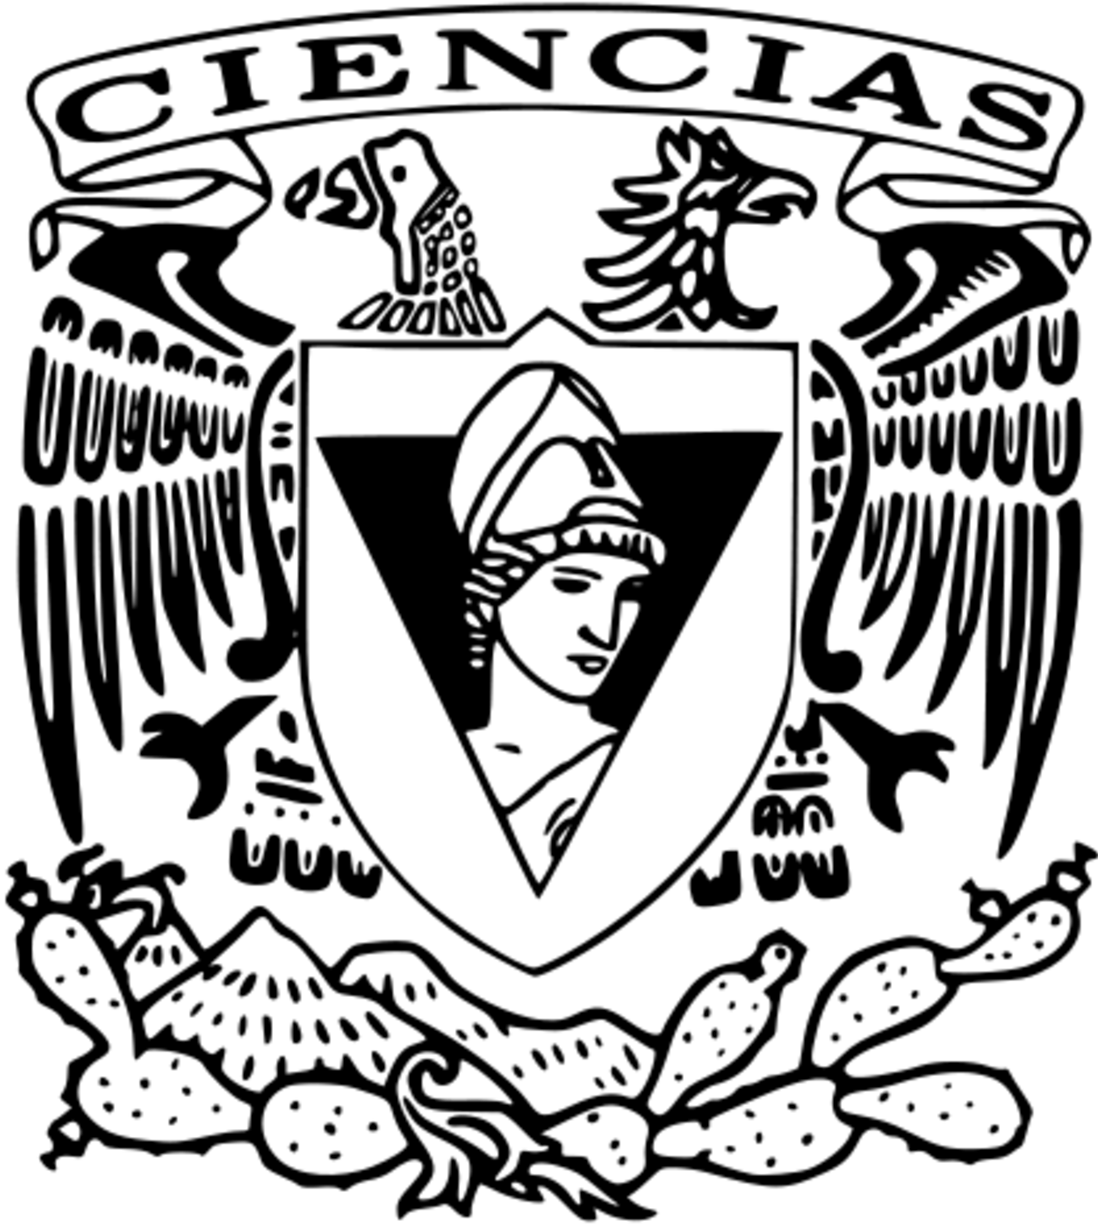
\includegraphics[height=3.4cm]{Logo_FC.png}
    	\end{center}
    \end{minipage}
\end{center}

\rule{17cm}{0.1mm}

%------ Fin de encabezado -------- %
\begin{tcolorbox}[
	title = \textcolor{black}{\textcolor{white}{Problema 2}},]
\textit{Sea $n\in \N$, $x_0=0$, $x_i>0$ para $i\in \N_n$ y $\sum_{i=1}^{n}\,x_i=1$, demuestre que:\,\\
\,\\
\begin{equation*}
    1\leq \sum_{i=1}^{n}\,\frac{x_i}{\sqrt{1+x_1+...+x_{i-1}}\,\,\sqrt{x_i+x_{i+1}+...+x_n}}<\frac{\pi}{2}
\end{equation*}
}
\end{tcolorbox}
\begin{proof}\,\\
    \,\\
    Definimos $y_i=\sum_{i=0}^i\,x_i$, reescribiendo obtenemos:\,\\
    \,\\
    \begin{equation*}
        \sum_{i=1}^{n}\,\frac{y_i-y_{i-1}}{\sqrt{1+y_{i-1}}\,\sqrt{1-y_{i-1}}}= \sum_{i=1}^{n}\,\frac{y_i-y_{i-1}}{\sqrt{1-(y_{i-1})^2}}
    \end{equation*}\,\\
    \,\\
     Ahora por la defininici\'on de $y_i$, se sigue que $0\leq y_i< 1$, para toda $i\in \N_n/\{n\}$
     la suma esta bien definida pues $1-(y_{i-1})^2>0$, ademas que $y_n=1$\,\\
     \,\\
    Tomemos $f:[0,1)\Rightarrow \R^+$, $f(x)=\frac{1}{\sqrt{1-x^2}}$, tenemos que
    como $f'(x)=\frac{x}{(1-x^2)^{\frac{3}{2}}}\geq 0$ para todo $x\in [0,1)$, por tanto $f$ es crciente
    en todo su dominio\,\\
    \,\\
    Consideramos la partici\'on $P$ de $[0,1]$, $P:=\{y_i\}_{i\in \N_n}$, del hecho de que 
    $f$ es creciente obtenemos que:\,\\
    \,\\
    \begin{equation*}
        \sum_{i=1}^{n}\,\frac{y_i-y_{i-1}}{\sqrt{1-(y_{i-1})^2}}=\underline{S}\,(P,f)
    \end{equation*}\,\\
    Finalmente obtenemos que\,\\
    \,\\
    \begin{equation*}
        \sum_{i=1}^{n}\,\frac{y_i-y_{i-1}}{\sqrt{1-(y_{i-1})^2}}<\int_{0}^{1}\,\frac{1}{\sqrt{1-x^2}}\,dx=\frac{\pi}{2}
    \end{equation*}\,\\
    \,\\
    \newpage
    \,\\
    Para la nueva desigualdad tenemos que $\sqrt{1-(y_{i-1})^2}<1$, por tanto tenemos que:\,\\
    \,\\
    \begin{equation*}
         1=\sum_{i=1}^{n}\,y_i-y_{i-1} < \sum_{i=1}^{n}\,\frac{y_i-y_{i-1}}{\sqrt{1-(y_{i-1})^2}}
    \end{equation*}
\end{proof}\,\\
\begin{tcolorbox}[
	title = \textcolor{black}{\textcolor{white}{Problema 3}},]
\textit{Si $X$ es un conjunto con una norma $\|.\|$ y que satisface que para todo $\epsilon$ existen $y_1,y_2,\cdots, y_n$
en $X$ tal que $X\subset \cup_{i=1}^{n}\,B(y_i,\epsilon)$. Pruebe que toda sucesi\'on en $X$ tiene una subsucesi\'on de Cauchy}
\end{tcolorbox}
\begin{proof}\,\\
    
\end{proof}\,\\
\begin{tcolorbox}[
	title = \textcolor{black}{\textcolor{white}{Problema 5}},]
\textit{Demuestre que existe una funci\'on derivable $f$ tal que $(f(x))^5+f(x)+x=0$ $\forall\,x\in \R$ y obtenga
$f'(x)$ $\forall\,x\in \R$
}
\end{tcolorbox}
\begin{proof}\,\\
    \,\\
    Sea $g:\R\rightarrow \R$ tal que $g(x)=-x^5-x$ como $g$ es continua y
    estrictacmente monotona, adem\'as de invertible tenemos que $g^{-1}$ es continua, luego como $g'(x)=-5x^4-1$, tenemos que $g´(x)\neq 0$ en todo $\R$,
    por tanto aplicando el teorema de la funci\'on inversa tenemos que $g^{-1}$ es derivable en $\R$, luego tenemos que:\,\\
    \,\\
    \begin{equation*}
        g\circ g^{-1}(x)=-(g^{-1}(x))^5-g^{-1}(x)=x\implies (g^{-1}(x))^5+g^{-1}(x)+x=0\,\,\,\forall x\in \R
    \end{equation*}\,\\
    Finalmente encontramos $g^{-1'}(x)$ para $x\in \R$:\,\\
    \,\\
    \begin{equation*}
        g^{-1'}(x)=\frac{1}{g'\circ g^{-1}(x)}=\frac{1}{-5(g^{-1}(x))^4-1}
    \end{equation*}
\end{proof}
\end{document}